% 力學 Project A2 實驗報告 — Group 22
% 編譯：xelatex report_G22.tex（需 xeCJK 與 Noto Serif/Sans CJK TC 字型；Overleaf 請選 XeLaTeX）
% 圖檔來源：../figures/（由 A2/run_all.py 產生）
\documentclass[11pt,a4paper]{article}

\usepackage{xeCJK}
\setCJKmainfont{Noto Serif CJK TC}
\setCJKsansfont{Noto Sans CJK TC}
\setCJKmonofont{Noto Sans CJK TC}
\xeCJKsetup{CJKecglue={\hskip 0.15em plus 0.05em}}

\usepackage[a4paper]{geometry}
\usepackage{amsmath,amssymb}
\usepackage{graphicx}
\usepackage{booktabs}
\usepackage{caption}
\usepackage{float}
\usepackage{hyperref}

\graphicspath{{../figures/}{figures/}}
\linespread{1.25}
\setlength{\parindent}{2em}
\captionsetup{font=small,labelfont=bf}
\renewcommand{\figurename}{圖}
\renewcommand{\tablename}{表}
\renewcommand{\contentsname}{目錄}

\newcommand{\dt}{\Delta t}

\title{力學 Project A2：單擺問題中\\velocity Verlet 與 RK4 的數值實驗}
\author{Group 22}
\date{2026 年 10 月}

\begin{document}
\maketitle

\section{研究目的與方法概要}

本報告執行 A1 中設計的四個數值實驗，比較 \textbf{velocity Verlet（以下簡稱 VV）}
與\textbf{四階 Runge--Kutta 法（RK4）}在單擺問題上的表現。實驗涵蓋兩組對照：
小角度近似與完整非線性方程、無阻尼與正比於角速度一次方的阻尼。

所有計算使用課程提供的數值工具包 \texttt{mechanics\_integrators.py}（未作任何修改），
程式與原始數據見 \texttt{A2/} 資料夾，執行 \texttt{python run\_all.py} 即可重現本報告所有圖表。

為了區分\textbf{物理現象}與\textbf{數值誤差}（A1 第 4 節），每個實驗都以 $\dt$ 與 $\dt/2$ 各跑一次：
\begin{itemize}
  \item 結果幾乎不隨 $\dt$ 改變 $\Rightarrow$ 屬於物理現象；
  \item 結果隨 $\dt$ 縮小，且縮小倍率約為 $2^p$（$p$ 為方法的收斂階數）$\Rightarrow$ 屬於數值誤差。
\end{itemize}
對 VV（二階）預期 $\dt$ 減半誤差縮為約 $1/4$；對 RK4（四階）預期約 $1/16$。

\section{物理模型與數值設定}

以 $\theta$ 為擺角、$\omega=\dot\theta$ 為角速度，取每單位質量，運動方程式為
\begin{align}
  \text{非線性：}\quad \ddot\theta &= -\frac{g}{L}\sin\theta - \gamma\,\omega, \\
  \text{小角度近似：}\quad \ddot\theta &= -\frac{g}{L}\,\theta - \gamma\,\omega ,
\end{align}
力學能（每單位質量）為
\begin{equation}
  E = \tfrac12 L^2\omega^2 + gL(1-\cos\theta)
  \qquad\left(\text{小角度模型以 } \tfrac12 gL\theta^2 \text{ 取代位能}\right).
\end{equation}

\begin{table}[H]
\centering
\caption{共用參數。初始角速度一律為 $0$。}
\begin{tabular}{lll}
\toprule
參數 & 數值 & 說明 \\
\midrule
$g$, $L$ & $9.8~\mathrm{m/s^2}$, $1~\mathrm{m}$ & $\omega_0=\sqrt{g/L}$，$T_0=2\pi/\omega_0=2.00709~\mathrm{s}$ \\
$\gamma$ & $0.3~\mathrm{s^{-1}}$ & 阻尼率（實驗三、四）；欠阻尼，衰減時間 $2/\gamma\approx 6.7~\mathrm{s}$ \\
$\dt$ & $0.01~\mathrm{s}$ 與 $0.005~\mathrm{s}$ & 每個實驗都跑兩種步長 \\
$\theta_0$ & 實驗一 $5^\circ$、$60^\circ$；實驗二、四 $120^\circ$；實驗三 $10^\circ$ & \\
\bottomrule
\end{tabular}
\end{table}

用來檢驗數值結果的精確參考值有兩個：
\begin{itemize}
  \item 無阻尼非線性單擺的精確週期 $T = 4K(k)/\omega_0$，$k=\sin(\theta_0/2)$，
        其中第一類完全橢圓積分以算術–幾何平均（AGM）計算：$K(k)=\pi/[2\,\mathrm{AGM}(1,\cos\frac{\theta_0}{2})]$。
  \item 有阻尼小角度單擺的解析解（$\omega_d=\sqrt{\omega_0^2-\gamma^2/4}$）：
  \begin{equation}
    \theta_{\text{exact}}(t)=\theta_0\,e^{-\gamma t/2}\left[\cos\omega_d t+\frac{\gamma}{2\omega_d}\sin\omega_d t\right].
  \end{equation}
\end{itemize}
週期由 $\theta(t)$ 由負轉正的過零點（線性內插）量測。

% ------------------------------------------------------------------
\section{實驗一：擺幅對週期的物理影響}

\textbf{設定：}無阻尼，固定使用 RK4，比較小角度近似與非線性方程，$\theta_0=5^\circ$ 與 $60^\circ$。

\begin{figure}[H]
\centering
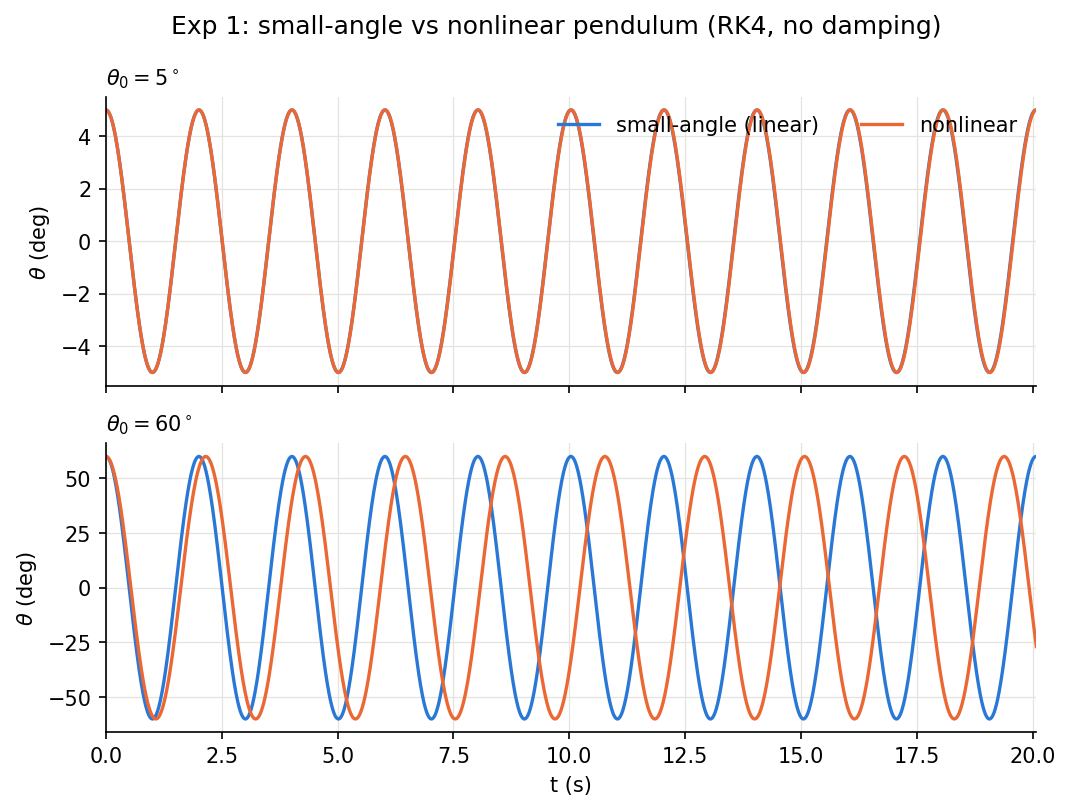
\includegraphics[width=0.82\textwidth]{exp1_theta_t.png}
\caption{實驗一：$\theta(t)$。上：$\theta_0=5^\circ$ 兩條曲線幾乎重合；下：$\theta_0=60^\circ$ 非線性解逐漸落後。}
\label{fig:exp1}
\end{figure}

\begin{table}[H]
\centering
\caption{實驗一量測到的平均週期（單位 s）。}
\begin{tabular}{cccccc}
\toprule
$\theta_0$ & 模型 & $T(\dt)$ & $|T(\dt)-T(\dt/2)|$ & 精確週期 & $T/T_0$ \\
\midrule
$5^\circ$  & 小角度 & 2.007090 & $6\times10^{-9}$ & 2.007090 & 1.0000 \\
$5^\circ$  & 非線性 & 2.008046 & $3\times10^{-8}$ & 2.008046 & 1.0005 \\
$60^\circ$ & 小角度 & 2.007090 & $6\times10^{-9}$ & 2.007090 & 1.0000 \\
$60^\circ$ & 非線性 & 2.153973 & $3\times10^{-8}$ & 2.153973 & 1.0732 \\
\bottomrule
\end{tabular}
\label{tab:exp1}
\end{table}

\textbf{結果與討論：}$5^\circ$ 時非線性週期只比 $T_0$ 長 $0.05\%$，兩條曲線肉眼無法區分；
$60^\circ$ 時週期變長 $7.3\%$，十個週期後兩者已幾乎反相（圖~\ref{fig:exp1}）。
$\dt$ 減半造成的週期變化只有 $10^{-8}~\mathrm{s}$ 量級，比 $60^\circ$ 的物理差異（$0.147~\mathrm{s}$）小了七個數量級，
且 RK4 結果與精確橢圓積分週期完全一致到小數點後六位。因此圖中的相位差\textbf{確實是物理現象}，與 A1 預測相符。

% ------------------------------------------------------------------
\section{實驗二：無耗散系統中的數值能量誤差}

\textbf{設定：}非線性方程、無阻尼、$\theta_0=120^\circ$（精確週期 $2.7555~\mathrm{s}$），模擬 $2000~\mathrm{s}$（約 726 個週期）。
物理上能量嚴格守恆，因此 $\Delta E/E_0$ 的任何變化都是數值誤差。

\begin{figure}[H]
\centering
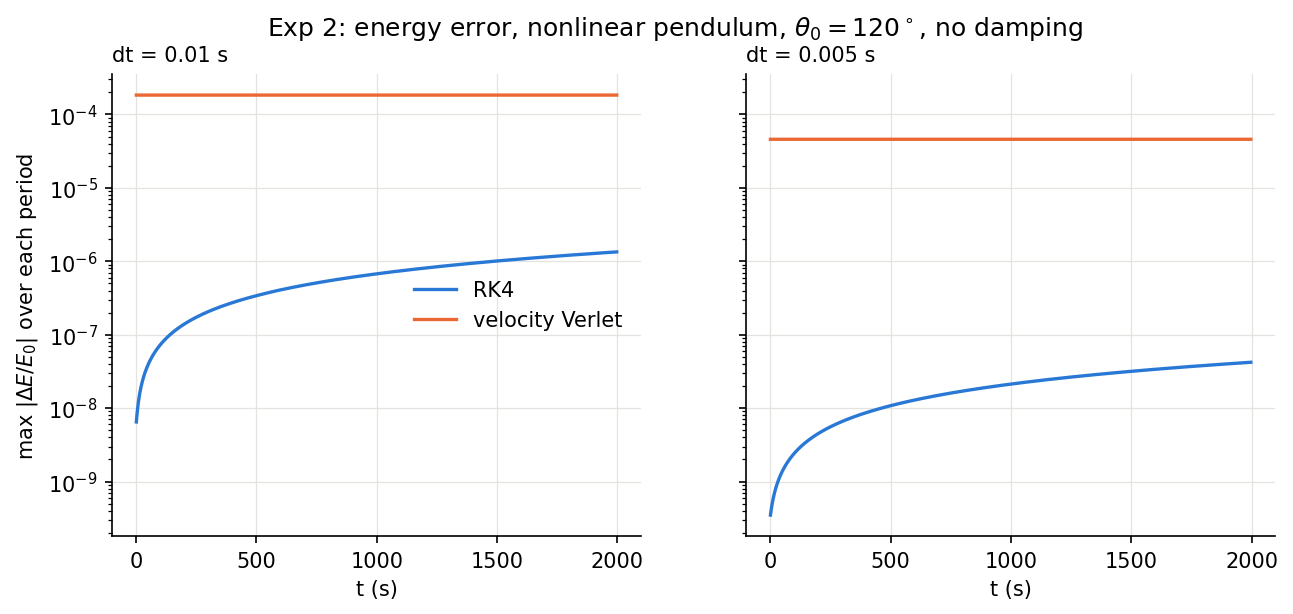
\includegraphics[width=0.95\textwidth]{exp2_energy_error.png}
\caption{實驗二：每個週期內 $|\Delta E/E_0|$ 的最大值（對數座標）。VV 誤差為固定寬度的有界震盪；RK4 誤差持續累積，但數值小得多。}
\label{fig:exp2}
\end{figure}

\begin{table}[H]
\centering
\caption{實驗二數值結果（$t_{\text{end}}=2000~\mathrm{s}$）。}
\begin{tabular}{lcccc}
\toprule
方法 & $\dt$ (s) & $\max|\Delta E/E_0|$ & 能量漂移率 (s$^{-1}$) & 週期誤差 (s) \\
\midrule
RK4 & 0.01  & $1.34\times10^{-6}$ & $-6.70\times10^{-10}$ & $-1.14\times10^{-6}$ \\
RK4 & 0.005 & $4.22\times10^{-8}$ & $-2.09\times10^{-11}$ & $-3.54\times10^{-8}$ \\
VV  & 0.01  & $1.84\times10^{-4}$ & （有界震盪，無漂移） & $-4.89\times10^{-5}$ \\
VV  & 0.005 & $4.59\times10^{-5}$ & （有界震盪，無漂移） & $-1.22\times10^{-5}$ \\
\midrule
\multicolumn{2}{l}{$\dt$ 減半之縮小倍率} & VV $4.0$；RK4 $31.9$ & RK4 $32$ & VV $4.0$；RK4 $32.3$ \\
\bottomrule
\end{tabular}
\label{tab:exp2}
\end{table}

\textbf{結果與討論：}
\begin{enumerate}
  \item \textbf{定性行為符合 A1 預測。}VV 的能量誤差在一個固定寬度內來回震盪，長時間不會累積，
        這是 symplectic 方法的特徵；RK4 的能量則\textbf{單調減少}，且隨時間線性累積，屬於數值耗散。
  \item \textbf{定量上與 A1 預測相反。}在 $\dt=0.01~\mathrm{s}$ 下，RK4 跑完 $2000~\mathrm{s}$ 的能量誤差
        （$1.3\times10^{-6}$）仍比 VV 的震盪幅度（$1.8\times10^{-4}$）\textbf{小約 140 倍}。
        以漂移率外推，RK4 要約 $2.7\times10^{5}~\mathrm{s}$（約 $10^5$ 個週期）才會追上 VV 的誤差帶。
        因此在一般模擬時間內，RK4 的能量反而比 VV 更準；VV 的優勢只有在極長時間或大步長下才顯現。
  \item \textbf{RK4 的能量流失率隨 $\dt^5$ 縮小，而非 A1 假設的 $\dt^4$。}
        實測 $\dt$ 減半時縮小 $32$ 倍。原因可由簡諧振子分析：RK4 每一步的放大因子滿足
        $|R(i z)|^2 = 1 - z^6/72 + z^8/576$（$z=\omega\dt$），
        即每步能量損失 $\propto \dt^6$，單位時間內步數 $\propto 1/\dt$，故流失率 $\propto \dt^5$。
        A1 中「$1/16$」的預估應修正為 $1/32$。VV 的能量誤差帶與週期誤差都恰好縮小 $4$ 倍，符合二階方法。
\end{enumerate}

為了讓 A1 預測的「相空間內縮」能被看見，另以刻意偏大的 $\dt=0.1~\mathrm{s}$ 重跑（圖~\ref{fig:exp2coarse}）：
$2000~\mathrm{s}$ 後 RK4 損失 $12.3\%$ 的能量，相空間軌跡明顯向內螺旋；
VV 誤差雖大（最大 $1.9\%$），但仍維持在固定帶內，軌跡閉合、不內縮。

\begin{figure}[H]
\centering
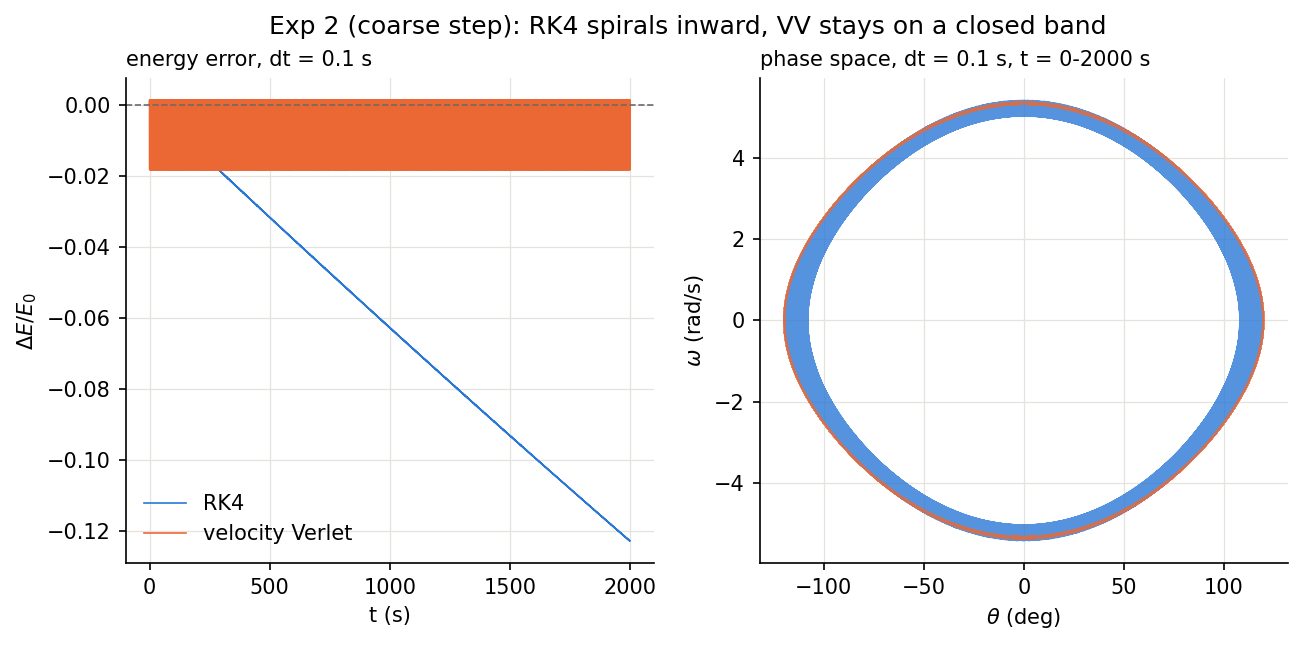
\includegraphics[width=0.95\textwidth]{exp2_phase_space_coarse.png}
\caption{實驗二（粗步長 $\dt=0.1~\mathrm{s}$）：左為 $\Delta E/E_0$，右為相空間軌跡 $(\theta,\omega)$。}
\label{fig:exp2coarse}
\end{figure}

% ------------------------------------------------------------------
\section{實驗三：有阻尼時的精確度比較}

\textbf{設定：}小角度近似、$\gamma=0.3~\mathrm{s^{-1}}$、$\theta_0=10^\circ$、模擬 $30~\mathrm{s}$，
將數值解與解析解 $\theta_{\text{exact}}(t)$ 比較。

\subsection{發現：工具包的 velocity Verlet 無法直接處理阻尼}

工具包的 \texttt{velocity\_verlet(acceleration, t, x0, v0)} 只接受 \texttt{acceleration(t, x)}，
加速度不能依賴速度（工具包 README 第 10 節）。實際把含阻尼的 \texttt{a(t, theta, omega)} 傳入時，程式直接報錯：
{\small
\begin{verbatim}
TypeError: accel_rk4.<locals>.a() missing 1 required positional argument: 'omega'
\end{verbatim}
}
這反映了一個本質問題：標準 VV 是為「只依賴位置的保守力」設計的。速度更新
$v_{n+1}=v_n+\frac{\dt}{2}(a_n+a_{n+1})$ 中的 $a_{n+1}$ 需要 $v_{n+1}$，而 $v_{n+1}$ 正是要求的量。
因此我們自行實作兩種修改版（工具包本身不修改），記 $f(\theta)$ 為重力造成的角加速度：
\begin{itemize}
  \item \textbf{延遲版（lagged）：}計算 $a_{n+1}$ 時沿用舊速度，
        $a_{n+1}\approx f(\theta_{n+1})-\gamma\,\omega_n$。這是最直覺的寫法。
  \item \textbf{隱式版（implicit）：}保留 $-\gamma\,\omega_{n+1}$ 並移項。由於阻尼對 $\omega$ 是線性的，可直接解出，無需迭代：
  \begin{equation}
    \omega_{n+1}=\frac{\omega_n+\frac{\dt}{2}\left[a_n+f(\theta_{n+1})\right]}{1+\gamma\dt/2}.
  \end{equation}
\end{itemize}
RK4 則以 \texttt{a(t, x, v)} 的一般形式自然處理阻尼，直接使用工具包。

\subsection{結果}

\begin{figure}[H]
\centering
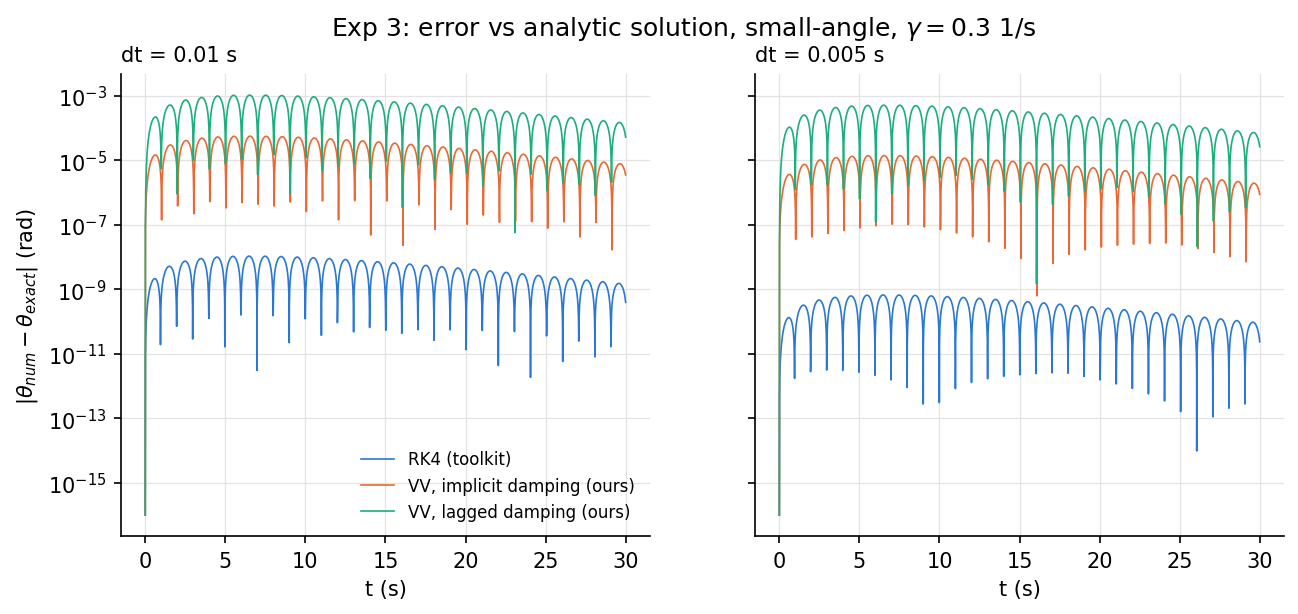
\includegraphics[width=0.95\textwidth]{exp3_error_vs_time.png}
\caption{實驗三：$|\theta_{\text{num}}-\theta_{\text{exact}}|$ 隨時間變化（對數座標）。}
\label{fig:exp3}
\end{figure}

\begin{figure}[H]
\centering
\begin{minipage}{0.52\textwidth}
\centering
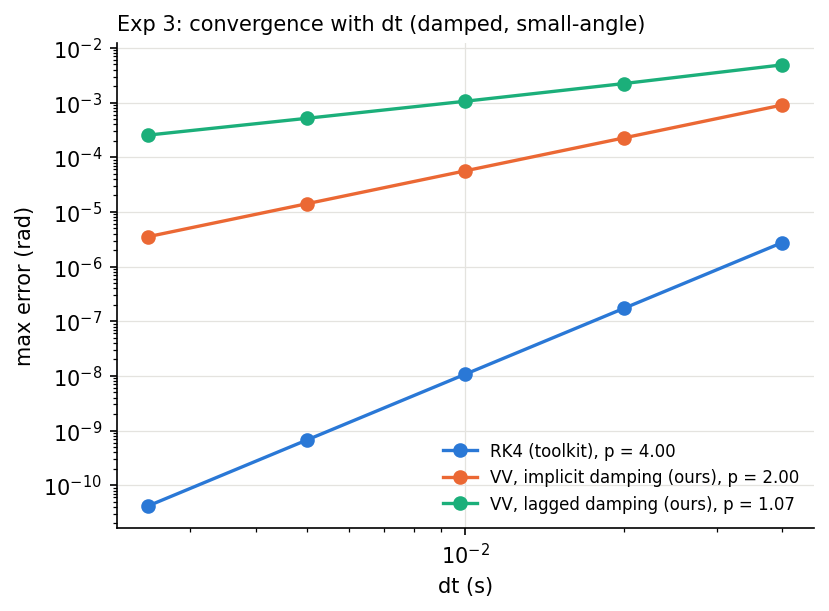
\includegraphics[width=\textwidth]{exp3_convergence.png}
\end{minipage}\hfill
\begin{minipage}{0.45\textwidth}
\centering
\small
\begin{tabular}{lccc}
\toprule
方法 & 最大誤差 & 減半倍率 & 階數 $p$ \\
\midrule
RK4         & $1.1\times10^{-8}$ & $16.0$ & $4.00$ \\
VV（隱式）  & $5.7\times10^{-5}$ & $4.0$  & $2.00$ \\
VV（延遲）  & $1.1\times10^{-3}$ & $2.1$  & $1.07$ \\
\bottomrule
\end{tabular}

\vspace{0.5em}
最大誤差為 $\dt=0.01~\mathrm{s}$、$0$--$30~\mathrm{s}$ 內的值（rad）；
階數 $p$ 由 $\dt=0.04$ 至 $0.0025~\mathrm{s}$ 五個步長擬合 誤差 $\propto\dt^p$。
\end{minipage}
\caption{實驗三：最大誤差對 $\dt$ 的收斂圖（左）與數值摘要（右）。}
\label{fig:exp3conv}
\end{figure}

\textbf{討論：}
\begin{enumerate}
  \item \textbf{延遲版 VV 只剩一階精度}（$p=1.07$），誤差最大。這正是 A1 預測的「處理速度變數的延遲」造成的殘差：
        每步在速度更新中引入 $O(\dt^2)$ 的誤差，累積後成為 $O(\dt)$。
  \item \textbf{隱式版 VV 恢復二階精度}（$p=2.00$），誤差比延遲版小約 20 倍。可見同樣叫「velocity Verlet」，
        處理速度相依力的方式會直接決定精度。
  \item \textbf{RK4 為四階}（$p=4.00$），誤差比隱式 VV 再小約 5000 倍，且不需修改演算法。
\end{enumerate}
三種方法的誤差都隨 $\dt$ 依各自階數縮小，因此全部屬於數值誤差；解析解與數值解的整體衰減行為一致。
此實驗符合 A1 預測，並補充了「工具包的 VV 介面不適用速度相依力」這項發現。

% ------------------------------------------------------------------
\section{實驗四：有阻尼時小角度近似與非線性方程的比較}

\textbf{設定：}$\gamma=0.3~\mathrm{s^{-1}}$、$\theta_0=120^\circ$、模擬 $30~\mathrm{s}$，使用 RK4。
有阻尼小角度單擺的週期為 $T_d=2\pi/\omega_d=2.00940~\mathrm{s}$。

\begin{figure}[H]
\centering
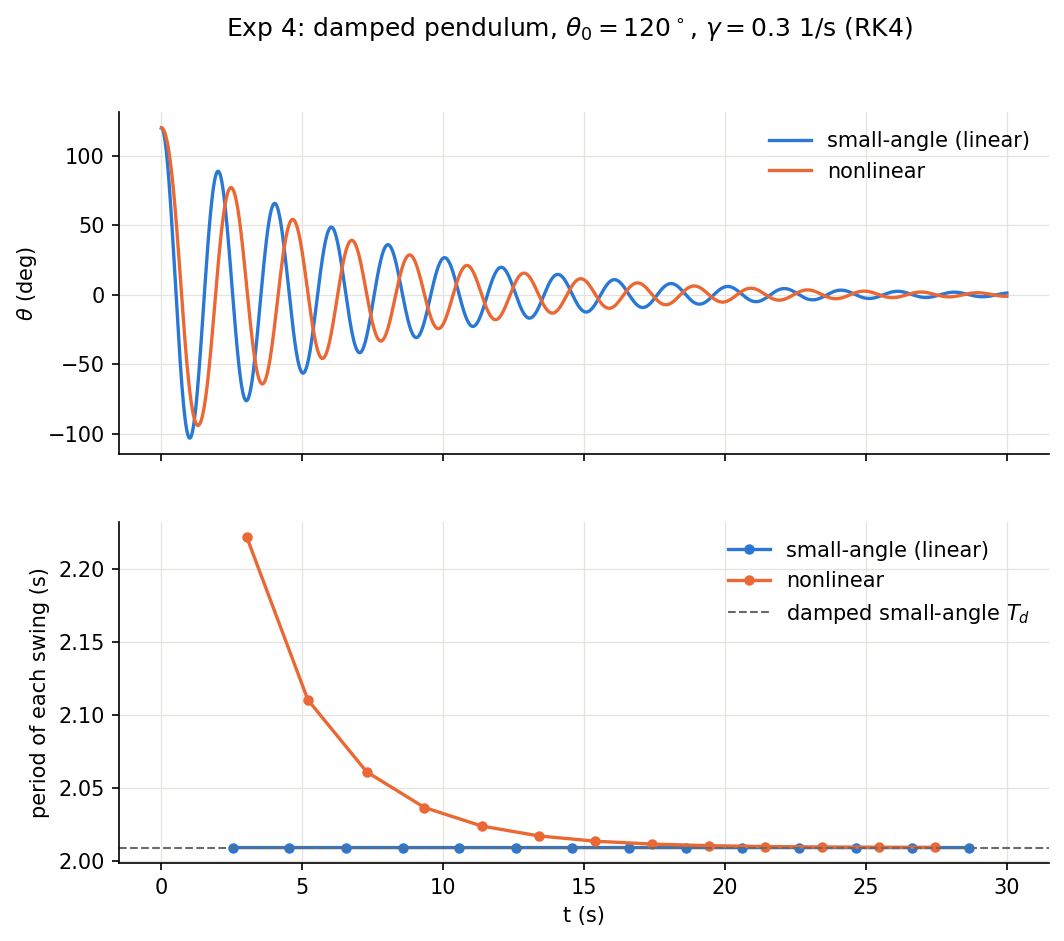
\includegraphics[width=0.82\textwidth]{exp4_theta_t_periods.png}
\caption{實驗四：上為 $\theta(t)$；下為每次擺動的週期，虛線為 $T_d$。}
\label{fig:exp4}
\end{figure}

\textbf{結果與討論：}
\begin{enumerate}
  \item \textbf{頻率收斂：}非線性單擺第一個週期為 $2.222~\mathrm{s}$（比 $T_d$ 長 $10.6\%$），
        隨振幅衰減依序為 $2.110$、$2.061$、$2.037$、$2.024~\mathrm{s}\ldots$，最後收斂到 $2.0095~\mathrm{s}\approx T_d$。
        小角度模型則從頭到尾維持 $T_d$。這與 A1 的預測一致：阻尼消耗能量使振幅變小，非線性效應隨之消失。
  \item \textbf{相位不會同步：}A1 預測兩者「最終同步停下」，但模擬顯示前期大振幅時累積的時間落後
        （最後一個共同擺動約 $0.82~\mathrm{s}$，相當於 $147^\circ$ 相位）\textbf{不會消失}。
        頻率相同後，相位差只會保持固定，不會被追回。兩條曲線最終都衰減到零，但並不重合。
  \item \textbf{此差異為物理現象：}$\dt$ 減半時兩模型的 $\theta(t)$ 最大變化僅約 $10^{-7}~\mathrm{rad}$，
        遠小於兩模型之間的差異。
\end{enumerate}

% ------------------------------------------------------------------
\section{綜合討論}

\subsection{與 A1 預測的比較}

\begin{table}[H]
\centering
\small
\caption{A1 預測與 A2 實測結果比較（$\dt=0.01~\mathrm{s}$）。}
\begin{tabular}{p{0.06\textwidth}p{0.28\textwidth}p{0.42\textwidth}p{0.12\textwidth}}
\toprule
實驗 & A1 預測 & A2 實測 & 判定 \\
\midrule
一 & $60^\circ$ 非線性週期明顯變長 & $T/T_0=1.073$；與精確週期一致；與 $\dt$ 無關 & 符合 \\
二 & RK4 能量流失、相空間內縮；VV 守恆 & 行為正確，但 RK4 能量誤差反而小約 140 倍；內縮需粗步長才可見 & 定性符合 \\
二 & $\dt$ 減半 RK4 能量流失縮為 $1/16$ & 實測 $1/32$（流失率 $\propto\dt^5$） & 需修正 \\
三 & VV 因速度延遲產生累積殘差；RK4 殘差極小 & 工具包 VV 無法使用；延遲版一階、隱式版二階、RK4 四階 & 符合並補充 \\
四 & 非線性頻率收斂至線性，兩者同步停下 & 頻率收斂至 $T_d$；但相位差 $0.82~\mathrm{s}$ 永久保留 & 部分符合 \\
\bottomrule
\end{tabular}
\end{table}

\subsection{守恆、耗散與非線性問題中選擇方法的考量}

\begin{itemize}
  \item \textbf{守恆力問題：}symplectic 的 VV 保證能量誤差有界、不隨時間累積，適合極長時間積分
        （如天體軌道、分子動力學）。但「有界」不等於「較小」：在中等時間尺度下，高階的 RK4 誤差可能小得多。
        選擇時應同時考慮模擬時間長度與所需精度，而不只看是否 symplectic。
  \item \textbf{耗散問題：}阻尼力依賴速度，標準 VV 不再適用，必須修改演算法，且修改方式會決定精度
        （一階或二階）；修改後 VV 也不再嚴格 symplectic。RK4 以一般的 $(x,v)$ 狀態形式自然處理，
        且物理上能量本來就在流失，RK4 微小的數值耗散相較於物理耗散可忽略。
  \item \textbf{非線性問題：}週期隨振幅改變，數值方法的週期（相位）誤差會與物理上的週期變化混在一起。
        必須以 $\dt$ 減半或精確週期等參考值確認觀察到的相位差來自物理，而非數值。
\end{itemize}

\section{結論}

\begin{enumerate}
  \item 以 $\dt$ 減半區分物理與數值誤差的方法有效：物理差異（週期變長、相位落後）與 $\dt$ 無關；
        數值誤差則依方法階數精確縮小（VV $\times1/4$、RK4 $\times1/16$，能量流失 $\times1/32$）。
  \item VV 在無耗散系統中確實能量不漂移，但在 $\dt=0.01~\mathrm{s}$、數百個週期內，RK4 的能量與週期誤差都更小。
  \item 工具包的 VV 無法直接處理阻尼；自行修改時，延遲處理速度只有一階精度，隱式處理可恢復二階。
        對於有阻尼的問題，RK4 是更自然且精確的選擇。
  \item 有阻尼的大角度單擺，頻率會收斂到小角度近似的頻率，但早期累積的相位差不會消失。
\end{enumerate}

\section{生成式 AI 使用說明}

本次作業中，生成式 AI（Claude）參與了以下工作：
閱讀課程工具包並說明其介面限制；依照本組 A1 的實驗設計撰寫 Python 實驗程式
（包含兩種修改版 velocity Verlet、精確週期與解析解的參考計算、週期量測與收斂分析）；
產生圖表與數值摘要；以及協助整理本報告的初稿。
實驗設計、參數選擇的確認與結果詮釋由組員檢查與討論。所有數值皆可由 \texttt{A2/run\_all.py} 重現。

\end{document}
